\documentclass[12pt]{article}
\usepackage[pdftex]{graphicx}   % assume PDFLaTeX
\usepackage{amsmath}

\textwidth = 6.5 in
\textheight = 9 in
\oddsidemargin = 0.0 in
\evensidemargin = 0.0 in
\topmargin = 0.0 in
\headheight = 0.0 in
\headsep = 0.0 in
%\parskip = 0.2in
\parskip 6pt
\parindent = 0.0in

%\textwidth 6.5in
%\textheight 9in
%\oddsidemargin 0pt
%\evensidemargin 0pt
%\topmargin -.5in
%\headheight .25in

\newtheorem{theorem}{Theorem}
\newtheorem{corollary}[theorem]{Corollary}
\newtheorem{definition}{Definition}
%% Add next two lines for Adobe type fonts! 12/5/01 Tony Seibert
\fontfamily{ptm}\selectfont
\renewcommand{\rmdefault}{ptm}

%\title{Brief Article}
%\author{The Author}
\begin{document}

%\ifpdf
%\DeclareGraphicsExtensions{.pdf, .jpg, .tif}
%\else
%\DeclareGraphicsExtensions{.eps, .jpg}
%\fi

\DeclareGraphicsExtensions{.pdf, .jpg, .tif}



\begin{center}
\section*{Lab 8: Synchronous Circuits}
UC Davis Physics 116B\\
\end{center}

\section*{Introduction}



In this lab, we will explore some basic ``synchronous" circuits; that is, circuits in which aggregate of logic states (bits) changes
changes with each subsequent clock cycles, based on their values in the previous clock cycle, and perhaps external (asynchronous)
inputs.

Pin-outs for the chips you might need for this lab are included in the Appendix.


\section *{Data Latch}

\begin{figure}[!h]
\centerline{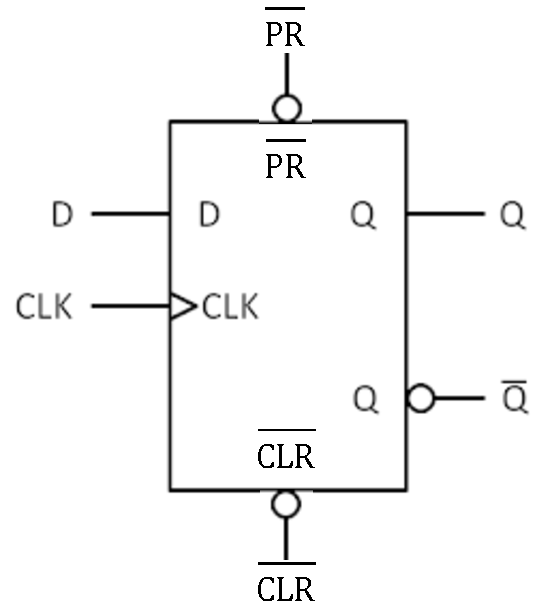
\includegraphics[width=2in]{figs/d-latch-7474.pdf}}
\caption{Standard data latch with asynchronous preset and clear.}
\label{fig:d-latch-7474}
\end{figure}


In addition to combinatorial logic, one of the fundamental building blocks of synchronous circuitry is the
data latch, which latches (or holds) the state of a bit on the rising edge of each clock cycle.
In a previous lab, you constructed these out of discrete gates, but a variety are available
as standard parts.  In this lab, you will use the 74LS74, which contains two data latches with the 
inputs and outputs shown in Figure~\ref{fig:d-latch-7474}.  In addition to the inputs we discussed in the previous section,
each of these has  asynchronous preset ($\overline{PR}$) and clear ($\overline{CLR}$) which will set or clear the output, regardless of the state of $D$ or $CLK$.

Wire up one of the flip-flops in the 74LS74 and verify that in behaves like the discrete data latch you built previously.  In addition,
verify that the $\overline{PR}$ and $\overline{CLR}$ inputs behave as expected.  Draw a time line to illustrate the operation, including the effect of all four inputs.

We will not be using the $\overline{PR}$ and $\overline{CLR}$ inputs for the rest of the lab, so be sure to tie them to +5V
to avoid spurious behavior!

\section*{The Simplest State Machine}

A ``state machine" is an important concept in synchronous logic design in which the states of a set of logic bits evolve with each clock edge ($CLK_i$) based on their
values at the previous clock edge ($CLK_{i-1}$) and possibly other inputs.

In this section, we will build the simplest possible non-trivial state machine\footnote{So simple most people wouldn't even call it a `state machine".}: a 1-bit state machine defined by $Q_{i}=\overline{Q_{i-1}}$; that is, the value of $Q$ toggles with each clock edge.  

Wire up the circuit shown in Figure~\ref{fig:toggler} and verify that it behaves this way.

\begin{figure}[!h]
\centerline{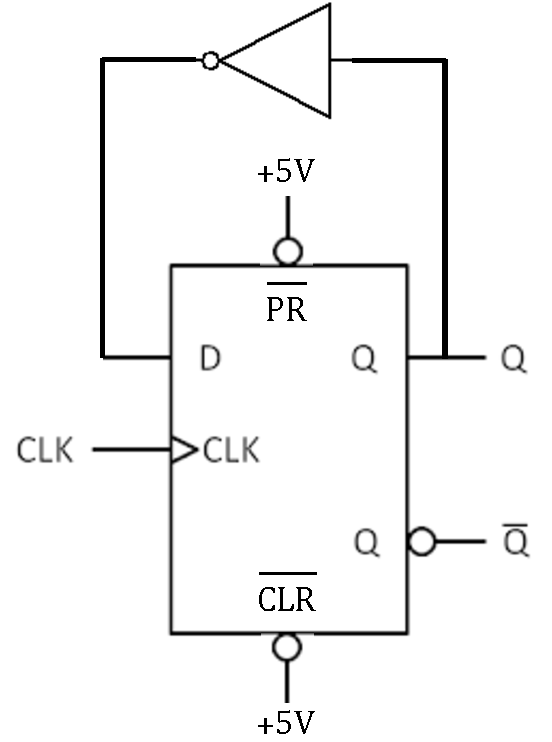
\includegraphics[width=2in]{figs/toggler.pdf}}
\caption{Circuit which will toggle the output state on each subsequent clock cycle.}
\label{fig:toggler}
\end{figure}

\section*{Shift Register}

\begin{figure}[!h]
\centerline{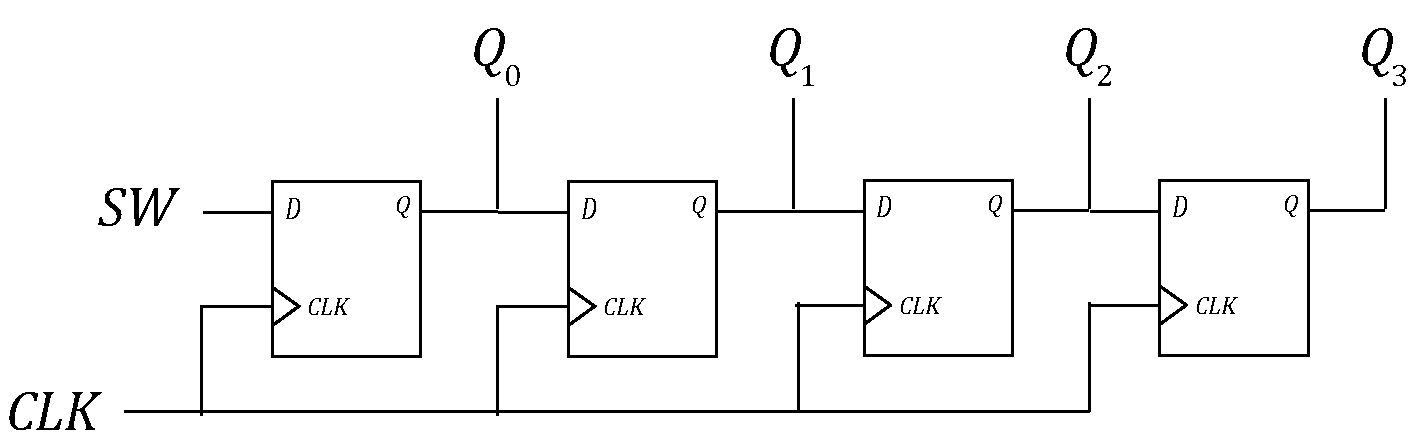
\includegraphics[width=6in]{figs/shift_register.pdf}}
\caption{Circuit which will toggle the output state on each subsequent clock cycle.}
\label{fig:shift_register}
\end{figure}


A ``shift register" shifts a bit from one location to the next on subsequent clock cycles.  Among other things, shift registers are a powerful
tool in translating back and forth between parallel and serial data. Wire up the shift register shown in Figure ~\ref{fig:shift_register}.  
Drive the common clock with the TTL pulser at a very low frequency ($<1$ Hz).  Connect the outputs to 4 LEDs, and the input of the first
shift register to one of the switches.  

Verify that you can manipulate the switch to cause a single bit to shift through the registers, then 2, then 3.

For your write-up, include a timeline of a single bit advancing through the four outputs (i.e., one time line for each $Q$).  

\section*{Synchronous Counter}

\begin{figure}[!h]

We discussed synchronous counters in class.  Wire up the counter shown in Figure~\ref{fig:counter} so that the outputs ($Q_3\rightarrow Q_0$) are
a binary count of clock cycles, with $Q_0$ being the lowest order bit.  The wiring for $Q_0$ is shown.  Determine the cominatorial logic necessary
to get the higher order bits to behave correctly.  Note, you might need to get a bit clever to wire the input to $Q_3$ with the gates in the Appendix.


\centerline{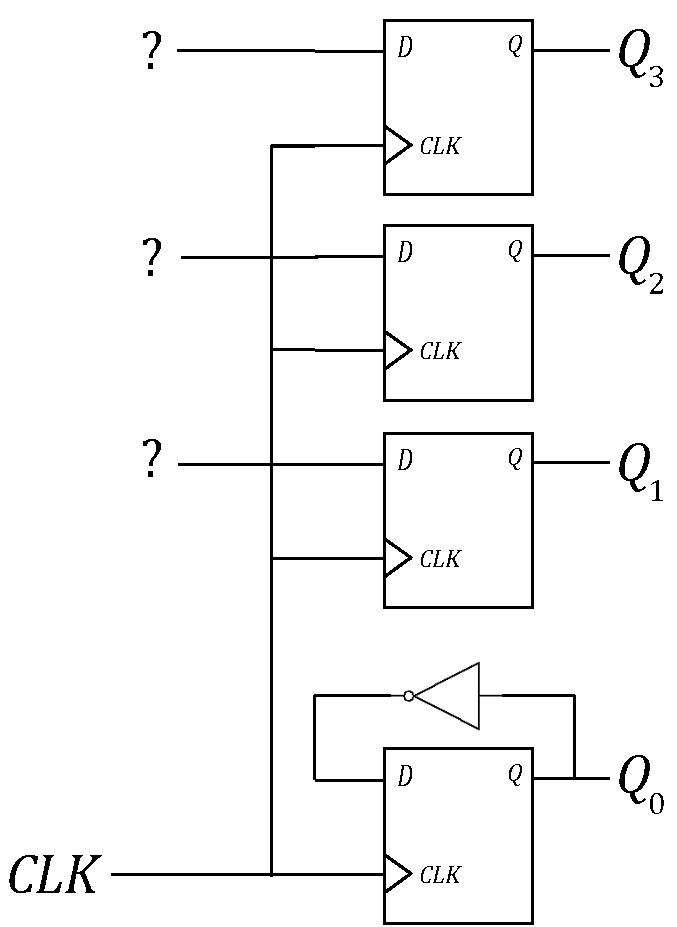
\includegraphics[width=2in]{figs/counter.pdf}}
\caption{Synchronous counter. Determine the logic you will need to make it function correctly.}
\label{fig:counter}
\end{figure}

Drive the circuit with a slow clock, and connect the outputs to LEDs.  Verify that it functions correctly.  For your lab writeup, include a schematic 
of your circuit, as well as a timeline to count from 0 to 15.

As a final step, increase the pulse rate ($\approx 1$ kHz), and determine the longest propagation delay between the clock and 
the change of state of one of the outputs.  Include the corresponding scope trace in your report.

\section*{Appendix:  Pinouts for Common Chips}

\vskip 1 cm

\centerline{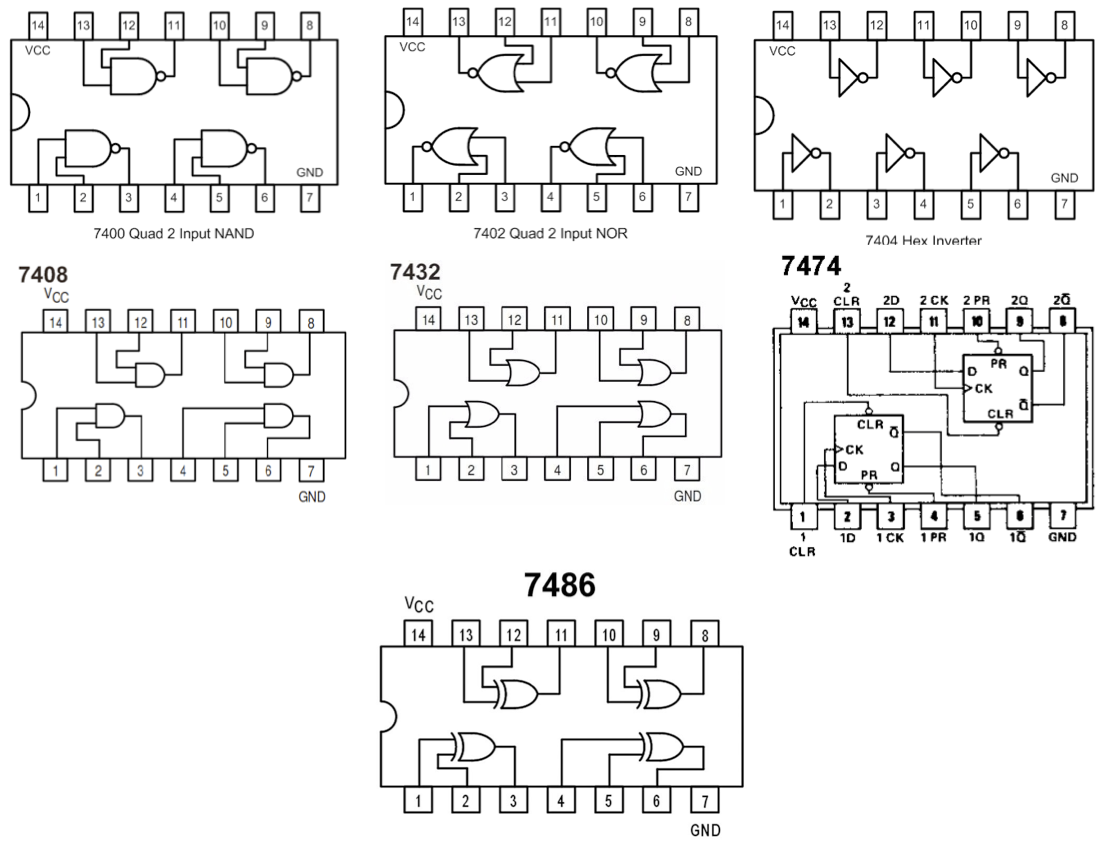
\includegraphics[width=6in]{figs/pinouts.png}}




\end{document}



